\documentclass[a4paper]{book}

\usepackage{amsmath,longtable,fancyhdr,booktabs,multirow,graphicx,float}
\usepackage{amssymb}
\usepackage{color}
\usepackage[colorlinks,
            linkcolor=black,
            anchorcolor=blue,
            citecolor=green
           ]{hyperref}
\usepackage[top=1in,bottom=1in,left=1.25in,right=1.25in]{geometry}
\usepackage{CJKnumb,titlesec,titletoc}
\usepackage{mnsymbol}
\usepackage{theorem}
\usepackage{algorithmicx}

\usepackage[nottoc]{tocbibind}
\def\ci{\perp\!\!\!\perp}
\pagestyle{fancy}
%% define some commands
\newcommand{\ud}{\mathrm{d}}
\newcommand{\e}{\varepsilon}
\newcommand{\up}{\mathrm}
\def\dbar{\mathrm{\mathchar'26\mkern-12mu d}}
\newcommand{\wave}{\scriptsize{\sim}}
\renewcommand{\bf}{\mathbf}
\renewcommand{\cal}{\mathcal}
\newcommand{\mbf}{\mathbf}
\newcommand{\mcal}{\mathcal}
\newcommand{\bb}{\mathbb}
\newcommand{\mbb}{\mathbb}
\newcommand{\imp}[1]{\textit{#1}}
\newcommand{\bs}{\boldsymbol}
\newcommand{\mbs}{\boldsymbol}

\DeclareMathOperator*{\argmin}{arg\,min}
\DeclareMathOperator*{\argmax}{arg\,max}
\def\dbar{\mathrm{\mathchar'26\mkern-12mu d}}
\newcommand{\norm}[1]{\left\lVert#1\right\rVert}

\newtheorem{problem}{Problem}
\newtheorem{lemma}{Lemma}
\newtheorem{theorem}{Theorem}
\newtheorem{corollary}{Corollary}
\newtheorem{remark}{Remark}
\newtheorem{observation}{Observation}
\newtheorem{proposition}{Proposition}
\newtheorem{assumption}{Assumption}

\newcommand{\figref}[1]{Fig\onedot~\ref{#1}}
\newcommand{\equref}[1]{Eq\onedot~\eqref{#1}}
\newcommand{\secref}[1]{Sec\onedot~\ref{#1}}
\newcommand{\tabref}[1]{Tab\onedot~\ref{#1}}
\newcommand{\thmref}[1]{Thm\onedot~\ref{#1}}
\newcommand{\prgref}[1]{Program~\ref{#1}}
\newcommand{\clmref}[1]{Claim~\ref{#1}}
\newcommand{\lemref}[1]{Lemma~\ref{#1}}
\newcommand{\propref}[1]{Prop\onedot~\ref{#1}}
\newcommand{\ptyref}[1]{Property\onedot~\ref{#1}}
\newcommand{\yangs}[1]{{\color{cyan}{\bf\sf [YS: #1]}}}
\newcommand{\yang}[1]{{\color{cyan}{\bf\sf [#1]}}}
\newcommand{\Ep}{\mcal{E}}
\newcommand{\Epp}{\widehat{\mcal{E}}_s^+[\mu]}
\newcommand{\Eln}{\widehat{\mcal{E}}_{\lambda,n}[\mu]}
\newcommand{\mup}{\widehat{\mu}_{(X,Y)}^+}
\newcommand{\muln}{\widehat{\mu}_{\lambda,n}}
\newcommand{\Hy}{\mcal{H}_{\mcal{Y}}}
\newcommand{\Hx}{\mcal{H}_{\mcal{X}}}
\newcommand{\HK}{\mcal{H}_{K}}
\newcommand{\HH}{\mcal{H}}
\newcommand{\XX}{\mcal{X}}
\newcommand{\YY}{\mcal{Y}}
\newcommand{\ZZ}{\mcal{Z}}
\newcommand{\BB}{\mcal{B}}
\newcommand{\zz}{\mbf{z}}
\newcommand{\xx}{\mbf{x}}
\newcommand{\yy}{\mbf{y}}
\newcommand{\CC}{\mcal{C}}
\newcommand{\hC}{\widehat{\mcal{C}}}
\def\eg{\emph{e.g}\onedot}
\def\Eg{\emph{E.g}\onedot}
\def\ie{\emph{i.e}\onedot}
\def\Ie{\emph{I.e}\onedot}
\def\cf{\emph{cf}\onedot}
\def\Cf{\emph{Cf}\onedot}
\def\etc{\emph{etc}\onedot}
\def\vs{\emph{vs}\onedot}
\def\wrt{w.r.t\onedot}
\def\dof{d.o.f\onedot}
\def\aka{a.k.a\onedot}
\def\iid{i.i.d\onedot}
\def\etal{\emph{et al}\onedot}

\title{Notes of PRML}
\author{Siyu Wang}
\date{August 2018}

\begin{document}

\maketitle
\chapter{Mathematical Foundations}

\chapter{Probabilistic Models}
\section{Graphical Models}
We shall find it highly advantageous to augment the analysis using diagrammatic representations of probability distributions, called \textit{probabilistic graphical models}. These offer several useful properties:
\begin{enumerate}
    \item They provide a simple way to visualize the structure of a probabilistic model and can be used to design and motivate new models.
    \item Insights into the properties of the model, including conditional independence properties, can be obtained by inspection of the graph.
    \item Complex computations, required to perform inference and learning in sophisticated models, can be expressed in terms of graphical manipulations, in which underlying mathematical expressions are carried along implicitly.
\end{enumerate}
\textit{nodes}: random variables. \textit{links}: probabilistic relationships between the variables.
\newline
\textit{Bayesan networks (directed graphical models)}, \textit{undirected graphical models}, \textit{factor graph}.

\subsection{Bayesian Networks}
Decomposition of a joint probability distribution:
\begin{equation}
    \tag{8.1} p(a, b, c) = p(c|a, b)p(b|a)p(a)
    \label{eq8.1}
\end{equation}
and the corresponding graphical model can be seen in figure\ref{GM1}.
\begin{figure}
\begin{minipage}{0.5\textwidth}
    \centering
    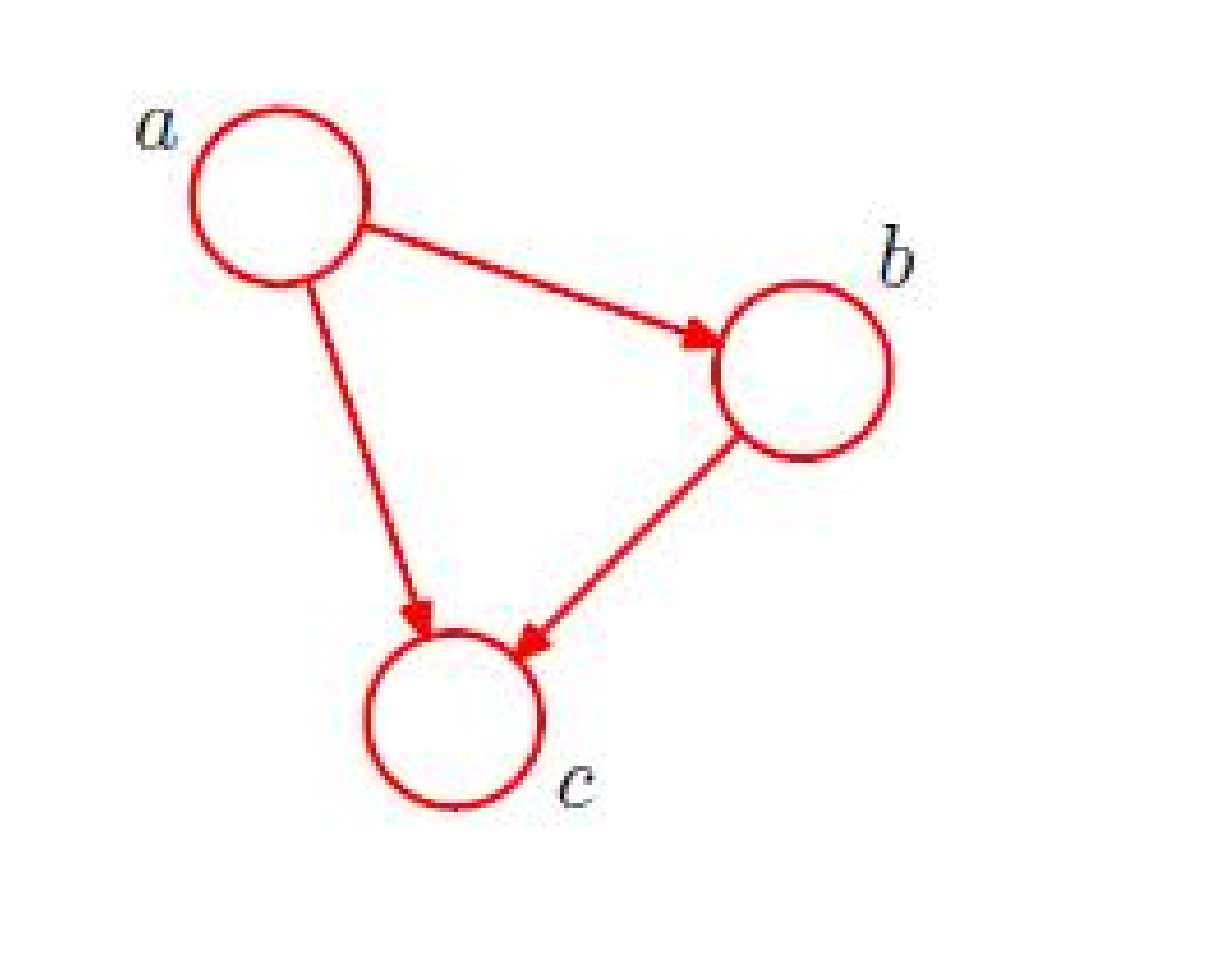
\includegraphics[width=0.5\linewidth]{./imgs/GM1.eps}
    \caption{}
    \label{GM1}
\end{minipage}
\begin{minipage}{0.5\textwidth}
    \centering
    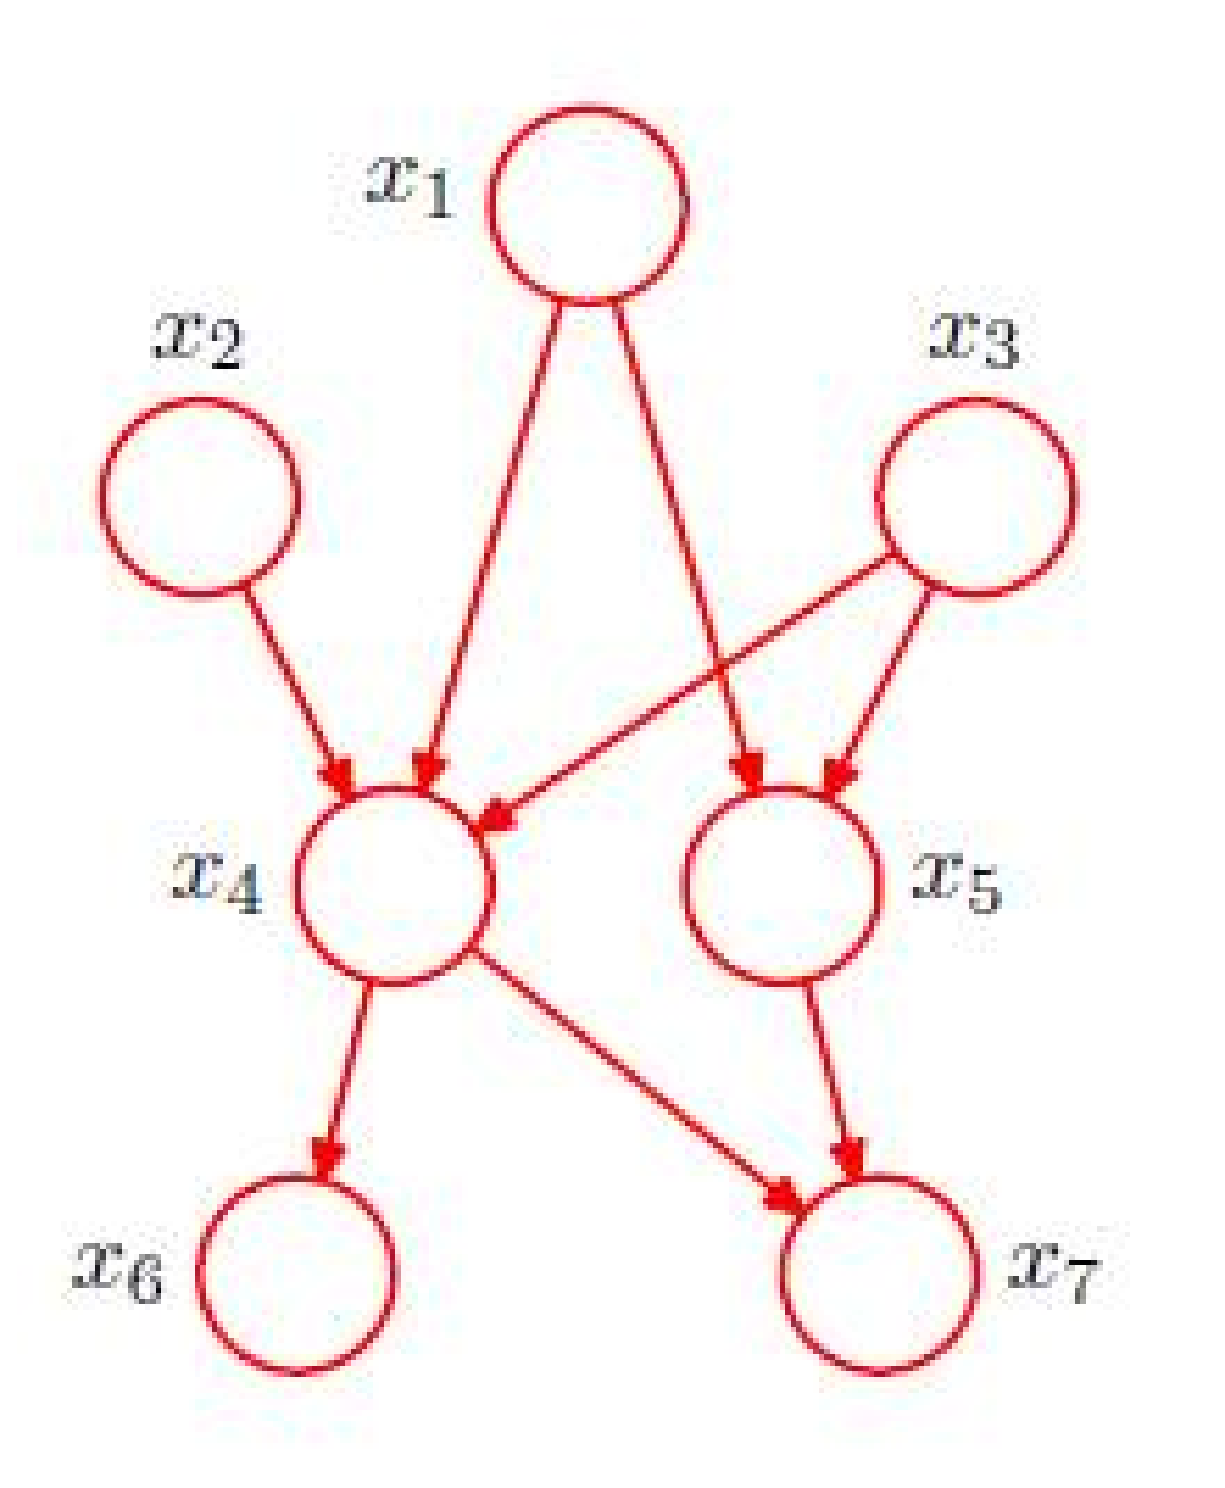
\includegraphics[width=0.5\linewidth]{./imgs/GM2.eps}
    \caption{}
    \label{GM2}
\end{minipage}
\end{figure}
\newline
\textbf{Rule}: for each conditional distribution we add directed links (arrows) to the graph from the nodes corresponding to the variables on which the distribution is conditioned.
\newline
we can extend the decomposition to $K$ variables:
\begin{equation}
    p(x_1,...,x_K) = p(x_K|x_1,...,x_{K-1})...p(x_2|x_1)p(x_1).
    \label{eq8.2}
\end{equation}
And the corresponding directed graph is called \textit{fully connected} because there is a link between every pair of nodes.
\newline
\textbf{Case} Given a directed graph as seen in \ref{GM2}, we can write the corresponding probability product:
\begin{equation}
    p(x_1)p(x_2)p(x_3)p(x_4|x_1,x_2,x_3)p(x_5|x_2,x_3)p(x_6|x_4)p(x_7|x_4,x_5)
    \label{8.3}
\end{equation}
\textbf{Rule}:
\begin{equation}
p(\textbf{x}) = \Pi_{k=1}^Kp(x_k|\mathrm{pa}_k)
\label{8.4}
\end{equation}
where $\mathrm{pa}_k$ denotes the set of parents of $x_k$, and $\textbf{x} = \{x_1,..,x_K\}$.
\newline
The directed graphs that we are considering are subject to an important restriction namely that there must be no \textit{directed cycles}, in other words there are no closed paths within the graph such that we can move from node to node along links following the direction of the arrows and end up back at the starting node. Such graphs are also called \textit{directed acyclic graphs}, or \textit{DAGs}. This is equivalent to the statement that there exists an ordering of the nodes such that there are no links that go from any node to any lower numbered node.
\subsubsection{Example: polynomial regression}
For more complex models, we shall adopt the convention that random variables will be denoted by open circles, and deterministic parameters will be denoted by smaller solid circles.
some concepts: \textit{observed variables, hidden variables, deterministic parameters}.
\subsubsection{Generative models}
\textit{sampling}: given a joint distribution, we want to draw a sample $\hat x_1, \hat x_2, ..., \hat x_K$ from it.
\textbf{ancestral sampling}
\newline
We start with the lowest-numbered node and draw a sample from the distribution $p(x_1)$, which we all $\hat x_1$. Then we work through each of the nodes in order, so that for node n we draw a sample from the conditional distribution p(xn|pan)
in which the parent variables have been set to their sampled values. Note that at each stage, these parent values will always be available because they correspond to lower-numbered
nodes that have already been sampled. The graphical model captures the \textit{causal} process by which the observed data was generated. For this reason, such models are often called \textit{generative} models. But the regression problem is not generative because there is no probability distribution associated with the input variable $x$, and it is not possible to generate synthetic data points from this model. But we can make it generative by introducing a suitable prior distribution $p(x)$, at the expense of a more complex model.
\subsubsection{Discrete variables}
\textit{parent-child pair in a directed graph. Two cases are particularly worthy of note, namely when the parent and child node each correspond to discrete variables and when they each correspond to Gaussian variables, because in these two cases the relationship can be extended hierarchically to construct arbitrarily complex directed acyclic graphs.}
\newline
\textbf{Case}:  discrete variable $\textbf{x}$ having $K$ possible states is given by
\begin{equation}\label{eq8.5}
  p(\bf{x}|\bf{mu}) =  \Pi_{k=1}^K\mu_k^{x_k}
\end{equation} governed by $\bf{\mu}$.
Suppose we have to discrete variables $\bf x_1, \bf x_2$, joint distribution can be written as
\begin{equation}\label{eq8.6}
  p(\bf x_1, \bf x_2|\bf{\mu})=\Pi_{k=1}^K\Pi_{k=1}^K\mu_{kl}^{x_{1k}x_{2l}}.
\end{equation}
$x_{1k}$ denotes the $k^{th}$ component of $\bf x_1$.
\newline
$K^2-1$ parameters. If we have $M$ variables, there is $K^M-1$ parameters, exponential with the num $M$.
\newline
Suppose $\bf x_1$ and $\bf x_2$ are independent. Each variable is then described by a separate multinomial distribution, and total number of parameters will be $2(K-1)$. If extend to $M$ variables, there will be $M(K-1)$ variables, linear growth.
\newline
\textbf{Generally case}: more links than independent variables but less links than a fully connected graph.
\newline
We can turn a graph over discrete variables into a Bayesian model by introducing Dirichlet priors for the parameters.
\newline
Another way of controlling the exponential growth in the number of parameters
in models of discrete variables is to use parameterized models for the conditional
distributions instead of complete tables of conditional probability values.
\subsubsection{Linear-Gaussian models}

\subsection{Conditional Independence}
If
\begin{equation}\label{eq8.7}
  p(a|b, c) = p(a|c),
\end{equation}
we say that $a$ is conditionally independent of $b$ given $c$, and we denote this by $$a\ci b|c .$$  And we will have
\begin{equation}\label{eq8.8}
  p(a,b|c) = p(a|c)p(b|c).
\end{equation}
\subsubsection{Examples}
Three examples related to conditional independence: \textit{tail-to-tail, head-to-tail, head-to-head}.
\subsubsection{D-separation}
We wish to ascertain whether a particular conditional
independence statement$$A\ci B |C$$is implied by a given directed acyclic graph.
\newline
i.i.d data points. Given $\mu$, we can say the data points $x_1,x_2,...,x_N$ are conditionally independent, but we can not say the data points are independent. because given $x_1$, the probability of $\mu$ will be affected and then $x_2$ will be affected.
\newline
\textbf{naive Bayes Model} Observation of $\bf{z}$ will block the path between $x_i$ and $x_j$ for $j\neq i$. So, if we are given a training set will, comprising inputs $\{x_1,...,x_N\}$ together with their labels, then we can fit the naive Bayes model to the training data using maximum likelihood assuming that the data are drawn independently from the model.
\newline
We can view a directed graph as a filter and all probability distribution $p(\bf x)$ that will be allowed through can make a set $\mathcal {DF}$.
\newline
\textbf{Markov blanket}.
\begin{equation}\label{eq8.9}
  p(\bf{x}_i|\bf{x}_{\{j\neq i\}}) = \frac{p(\bf x_1,...\bf x_D)}{\int p(\bf x_1,...,\bf x_D)\rm d\bf x_i}=\frac{\prod_k p(\bf x_k|\rm{pa}_k)}{\int \prod_k p(\bf x_k|\rm{pa}_k)\rm{d}\bf x_i}
\end{equation}
Some factors in $\prod_k p(\bf x_k|\rm{pa}_k)$ will disappear if they are not relative to $\bf x_i$.
\subsection{Markov Random Fields}

\subsection{Inference in Graphical Models}
\end{document} 